\section{Generalized Linear Models and Generalized Additive Models}
\begin{frame}
\huge{\centerline{Section 4: Generalized Linear Models }}
\huge{\centerline{and Generalized Additive Models}}
\end{frame}

\begin{frame}
\frametitle{Generalized Linear Models (GLM)}
\begin{itemize}
\item Generalized Linear Models are models in which conditional distribution of the response falls in some parametric family (exponential family), and the parameters are set by the linear predictor.
\item Link function determines the relationship between the parameters and the linear predictor.
\item Usually $g(E(\textbf{Y}))=g(\textbf{$\mu$})=\textbf{$X$}\textbf{$\theta_1$}+\textbf{$\theta_0$}$, where g is the link function.
\end{itemize}
\end{frame}

\begin{frame}
\frametitle{Generalized Linear Models (GLM) }
\begin{itemize}
\item Both least-squares regression and logistic regression are part of generalized linear models. 
\item Least-squares regression assumes gaussian distribution with mean predicted by the linear predictor. (identity link)
\item Logistic regression assumes binomial distribution, with $n$ equal to the number of data points with given $x$, and $p$ given by the logistic function. $(p=\frac{1}{1+e^{-(\theta_0+x \cdot \theta_1)}})$
\end{itemize}
\end{frame}
%\begin{frame}
%\frametitle{Linear Predictors}
%\begin{itemize}
%\item Maybe we don't need the slide
%\end{itemize}
%\end{frame}

% \begin{frame}
% \frametitle{Link Function}
% \begin{itemize}
% \item Link function determines the relationship between the parameters and the linear predictor.
% \item For GLM, link function may be any monotonic differentiable function. 
% \end{itemize}
% \end{frame}

\begin{frame}
\frametitle{GLM vs LM}
Data is generated with the the equation $y\sim \mathcal{N}(\mu, 0.5)$, $\mu=\frac{1}{0.4x}$.
\begin{figure}
\centering
\begin{subfigure}{.5\textwidth}
  \centering
  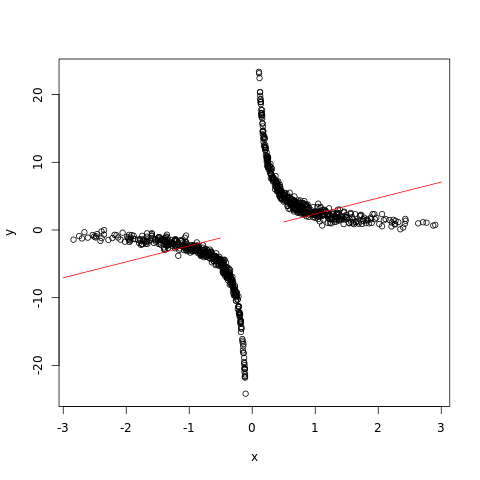
\includegraphics[height=.5\textheight]{glm/Unknown-2}
  \caption{Line fitted with least regression}
  \label{fig:sub1}
\end{subfigure}%
\begin{subfigure}{.5\textwidth}
  \centering
  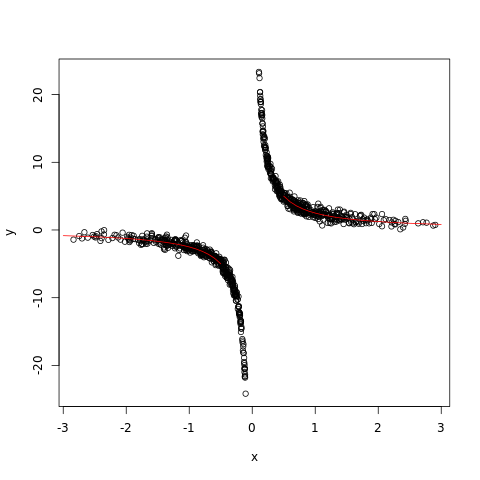
\includegraphics[height=.5\textheight]{glm/Unknown3}
  \caption{Line fitted with GLM}
  \label{fig:sub2}
\end{subfigure}
\label{fig:test}
\end{figure}
\end{frame}

\begin{frame}
\frametitle{Generalized Additive Models (GAM) }
\begin{itemize}
\item Unlike Generalized Linear Models, instead of making the transformed mean a linear function of the inputs, we can make it an additive function of the inputs
\item $g(E(\textbf{Y}))=g(\textbf{$\mu$})=\alpha + f_1(x_1) + f_2(x_2) + ... + f_n(x_n)$
\end{itemize}
\end{frame}

\begin{frame}
\frametitle{Model Checking}
\begin{itemize}
\item When our GLM is wrong, then no matter how much data we use, the prediction of our model is systematically wrong. However, since GAM can be nonparametric, with enough data, GAM will fit better than GLM. We can therefore use this property to design a procedure that detect if our GLM is wrong.
\end{itemize}
\end{frame}

\begin{frame}
\frametitle{Model Checking}
$MSE$: Mean Squared Error \\
$MSE_{p}$: Parametric mean squared error \\
$MSE_{np}$: Nonparametric \\
\begin{enumerate}
\item Fit a GAM and a GLM to the same data. Compute $MSE_p$ and $MSE_{np}$. Compute $t = MSE_p - MSE_{np}$.
\item Simulate from fitted GLM, refit both models to the simulated data. Repeat many times. compute $\hat{MSE_p}$ and $\hat{MSE_{np}}$. Compute $\hat{t} = \hat{MSE_p} - \hat{MSE_{np}}$.
\item p-value: $\frac{1 + \#\{\hat{t} > t\}}{1+\#\hat{t}}$
\end{enumerate}
\end{frame}

\begin{frame}
\frametitle{Model Checking: Example}
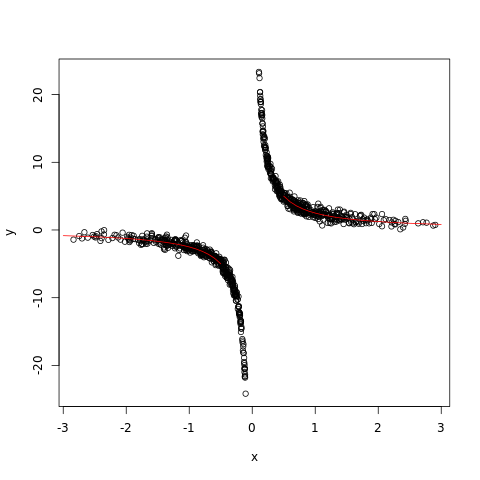
\includegraphics[height=.5\textheight]{glm/Unknown3}
\begin{itemize}
\item By performing model checking on our glm model with inverse link function, we get p-value of 0.72. This is reassuring, since the data is indeed generated from the inverse of a linear function.
\end{itemize}
\end{frame}

% \begin{frame}
% \frametitle{Trivia}
% \begin{itemize}
% \item Note that when the training data is perfectly linearly separable, maximum likelihood works badly for GLM.
% \end{itemize}
% \end{frame}